% Fig. 2 -- outdoor identity consistency (real data, ego frame).
% Paste-ready TikZ body. Include from sec/*.tex with:  % Fig. 2 -- outdoor identity consistency (real data, ego frame).
% Paste-ready TikZ body. Include from sec/*.tex with:  % Fig. 2 -- outdoor identity consistency (real data, ego frame).
% Paste-ready TikZ body. Include from sec/*.tex with:  % Fig. 2 -- outdoor identity consistency (real data, ego frame).
% Paste-ready TikZ body. Include from sec/*.tex with:  \input{figs/fig2_identity_consistency_body}
% Preamble requirements (main.tex already loads amsmath,amssymb,tikz,graphicx):
\usetikzlibrary{positioning, arrows.meta, backgrounds, fit}
%
% Drawn at 17.3cm == \textwidth (6.875in = 17.46cm), so NO \resizebox is used and
% every label typesets at its true point size. Do not wrap this in \resizebox.

\definecolor{idred}{HTML}{E41A1C}
\definecolor{idblue}{HTML}{377EB8}
\definecolor{idgreen}{HTML}{4DAF4A}
\definecolor{idpurple}{HTML}{984EA3}
\definecolor{boxbg}{HTML}{F8F9FA}
\definecolor{bordergray}{HTML}{D1D5DB}

\begin{figure*}[t]
\centering
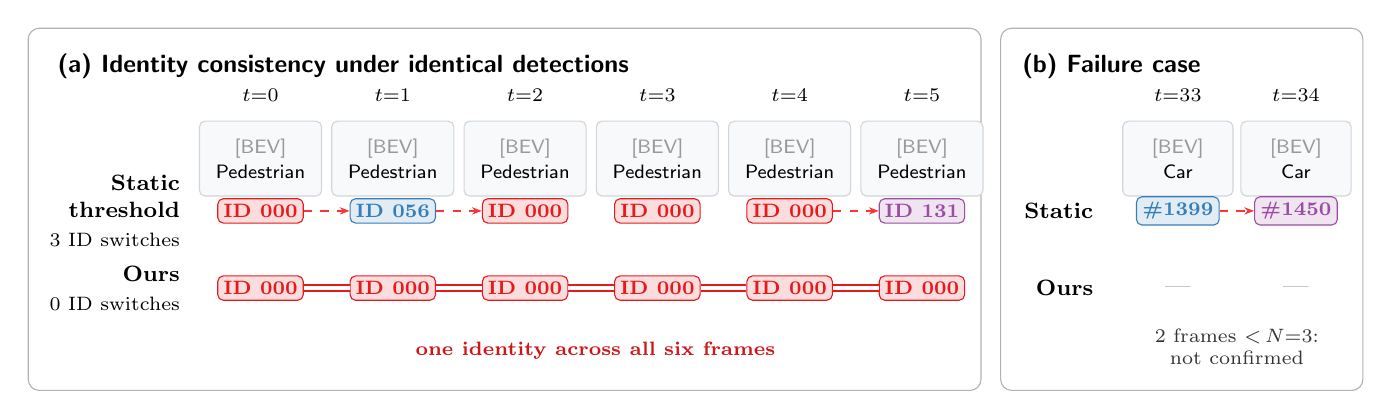
\begin{tikzpicture}[
    font=\small\sffamily,
    framebox/.style={draw=bordergray, fill=boxbg, rounded corners=2pt, minimum width=1.55cm, minimum height=0.95cm, align=center, inner sep=2pt},
    tagred/.style={fill=idred!15, text=idred, draw=idred, font=\scriptsize\bfseries, rounded corners=2pt, inner sep=2pt, minimum width=1.05cm, align=center},
    tagblue/.style={fill=idblue!15, text=idblue, draw=idblue, font=\scriptsize\bfseries, rounded corners=2pt, inner sep=2pt, minimum width=1.05cm, align=center},
    tagpurple/.style={fill=idpurple!15, text=idpurple, draw=idpurple, font=\scriptsize\bfseries, rounded corners=2pt, inner sep=2pt, minimum width=1.05cm, align=center},
    subpanel/.style={draw=black!30, fill=white, rounded corners=4pt}
]
% ---------------- panel (a) : 0 .. 12.2 ----------------
\node[anchor=north west, font=\small\sffamily] (titleA) at (0.25, -0.2) {\textbf{(a) Identity consistency under identical detections}};
\node[anchor=east, align=right, font=\footnotesize] (lblStaticA) at (2.05, -2.32) {\textbf{Static}\\\textbf{threshold}\\[1pt]{\scriptsize 3 ID switches}};
\node[anchor=east, align=right, font=\footnotesize] (lblOursA)   at (2.05, -3.30) {\textbf{Ours}\\[1pt]{\scriptsize 0 ID switches}};
\foreach \i/\t in {0/{$t{=}0$}, 1/{$t{=}1$}, 2/{$t{=}2$}, 3/{$t{=}3$}, 4/{$t{=}4$}, 5/{$t{=}5$}} {
    \node[anchor=center, font=\scriptsize\bfseries] (timeA\i) at (2.95 + \i*1.68, -0.85) {\t};
    \node[framebox, below=0.12cm of timeA\i] (frameA\i) {
        \textcolor{gray!80}{\scriptsize [BEV]}\\[-2pt]
        \scriptsize Pedestrian
    };
}
\node[tagred]    (s0) at (frameA0 |- lblStaticA) {ID 000};
\node[tagblue]   (s1) at (frameA1 |- lblStaticA) {ID 056};
\node[tagred]    (s2) at (frameA2 |- lblStaticA) {ID 000};
\node[tagred]    (s3) at (frameA3 |- lblStaticA) {ID 000};
\node[tagred]    (s4) at (frameA4 |- lblStaticA) {ID 000};
\node[tagpurple] (s5) at (frameA5 |- lblStaticA) {ID 131};
\draw[-{Stealth[length=3.5pt]}, dashed, red!80, line width=0.8pt] (s0) -- (s1);
\draw[-{Stealth[length=3.5pt]}, dashed, red!80, line width=0.8pt] (s1) -- (s2);
\draw[-{Stealth[length=3.5pt]}, dashed, red!80, line width=0.8pt] (s4) -- (s5);
\node[tagred] (o0) at (frameA0 |- lblOursA) {ID 000};
\node[tagred] (o1) at (frameA1 |- lblOursA) {ID 000};
\node[tagred] (o2) at (frameA2 |- lblOursA) {ID 000};
\node[tagred] (o3) at (frameA3 |- lblOursA) {ID 000};
\node[tagred] (o4) at (frameA4 |- lblOursA) {ID 000};
\node[tagred] (o5) at (frameA5 |- lblOursA) {ID 000};
\draw[double, double distance=1.2pt, idred, line width=0.9pt] (o0) -- (o1) -- (o2) -- (o3) -- (o4) -- (o5);
\node[anchor=center, font=\scriptsize\bfseries\color{idred!90!black}] (noteA) at (7.15, -4.10) {$\checkmark$ one identity across all six frames};
% ---------------- panel (b) : 12.45 .. 17.3 ----------------
\node[anchor=north west, font=\small\sffamily] (titleB) at (12.50, -0.2) {\textbf{(b) Failure case}};
\node[anchor=east, align=right, font=\footnotesize] (lblStaticB) at (13.65, -2.32) {\textbf{Static}};
\node[anchor=east, align=right, font=\footnotesize] (lblOursB)   at (13.65, -3.30) {\textbf{Ours}};
\node[anchor=center, font=\scriptsize\bfseries] (timeB0) at (14.60, -0.85) {$t{=}33$};
\node[anchor=center, font=\scriptsize\bfseries] (timeB1) at (16.10, -0.85) {$t{=}34$};
\node[framebox, minimum width=1.40cm, below=0.12cm of timeB0] (fb0) {\textcolor{gray!80}{\scriptsize [BEV]}\\[-2pt]\scriptsize Car};
\node[framebox, minimum width=1.40cm, below=0.12cm of timeB1] (fb1) {\textcolor{gray!80}{\scriptsize [BEV]}\\[-2pt]\scriptsize Car};
\node[tagblue,   minimum width=1.05cm] (sb0) at (fb0 |- lblStaticB) {\#1399};
\node[tagpurple, minimum width=1.05cm] (sb1) at (fb1 |- lblStaticB) {\#1450};
\draw[-{Stealth[length=3.5pt]}, dashed, red!80, line width=0.8pt] (sb0) -- (sb1);
\node[text=gray!70, font=\small] (ob0) at (fb0 |- lblOursB) {\textemdash};
\node[text=gray!70, font=\small] (ob1) at (fb1 |- lblOursB) {\textemdash};
\node[anchor=center, align=center, font=\scriptsize\color{black!80}] (noteB) at (15.35, -4.05) {2 frames ${<}\,N{=}3$:\\ not confirmed};
\begin{scope}[on background layer]
    \draw[subpanel] (0, 0) rectangle (12.10, -4.6);
    \draw[subpanel] (12.35, 0) rectangle (16.95, -4.6);
\end{scope}
\end{tikzpicture}
\caption{\textbf{Identity consistency under identical detections} (nuScenes \emph{val}, sensor frame, detection-budget-matched arms; dashed red arrows mark identity switches).
\textbf{(a)} One pedestrian in \texttt{scene-0925} over six consecutive keyframes. The emitted 3D box is identical in both arms in every frame --- same centre, size, orientation and score (0.726--0.833, centre error $\le 0.27$\,m, correctly classified throughout) --- so the two rows differ only in the identity attached to that box. The static score threshold assigns three distinct identities, returning to the first one in between; confirmation-based initialisation with retrospective emission assigns one.
\textbf{(b)} The corresponding cost: a correctly classified, well-localised car in \texttt{scene-0104} visible for only two keyframes, one short of the $N{=}3$ confirmation window. The threshold emits it, already split across two identities; our policy does not emit it at all.}
\label{fig:identity_consistency}
\end{figure*}

% Preamble requirements (main.tex already loads amsmath,amssymb,tikz,graphicx):
\usetikzlibrary{positioning, arrows.meta, backgrounds, fit}
%
% Drawn at 17.3cm == \textwidth (6.875in = 17.46cm), so NO \resizebox is used and
% every label typesets at its true point size. Do not wrap this in \resizebox.

\definecolor{idred}{HTML}{E41A1C}
\definecolor{idblue}{HTML}{377EB8}
\definecolor{idgreen}{HTML}{4DAF4A}
\definecolor{idpurple}{HTML}{984EA3}
\definecolor{boxbg}{HTML}{F8F9FA}
\definecolor{bordergray}{HTML}{D1D5DB}

\begin{figure*}[t]
\centering
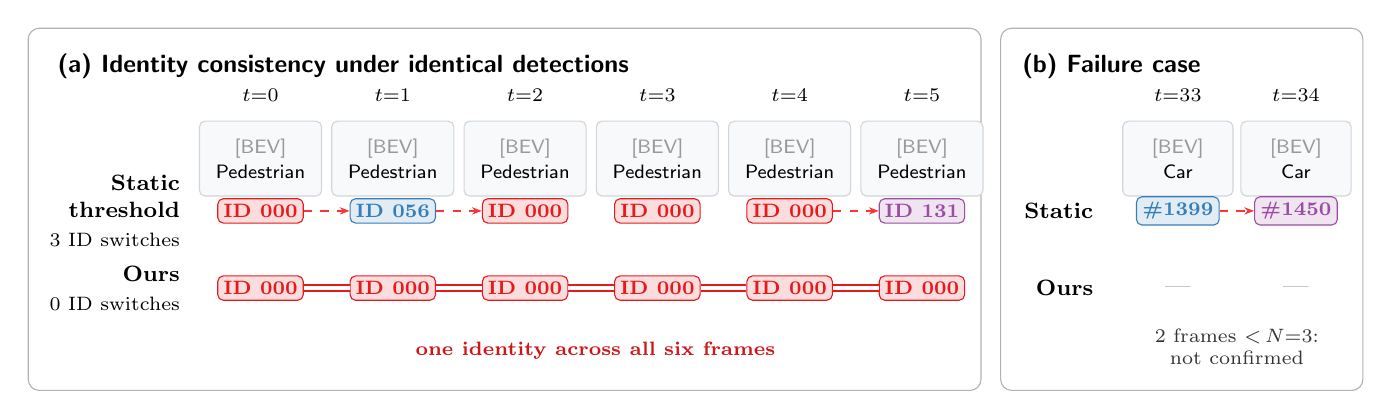
\begin{tikzpicture}[
    font=\small\sffamily,
    framebox/.style={draw=bordergray, fill=boxbg, rounded corners=2pt, minimum width=1.55cm, minimum height=0.95cm, align=center, inner sep=2pt},
    tagred/.style={fill=idred!15, text=idred, draw=idred, font=\scriptsize\bfseries, rounded corners=2pt, inner sep=2pt, minimum width=1.05cm, align=center},
    tagblue/.style={fill=idblue!15, text=idblue, draw=idblue, font=\scriptsize\bfseries, rounded corners=2pt, inner sep=2pt, minimum width=1.05cm, align=center},
    tagpurple/.style={fill=idpurple!15, text=idpurple, draw=idpurple, font=\scriptsize\bfseries, rounded corners=2pt, inner sep=2pt, minimum width=1.05cm, align=center},
    subpanel/.style={draw=black!30, fill=white, rounded corners=4pt}
]
% ---------------- panel (a) : 0 .. 12.2 ----------------
\node[anchor=north west, font=\small\sffamily] (titleA) at (0.25, -0.2) {\textbf{(a) Identity consistency under identical detections}};
\node[anchor=east, align=right, font=\footnotesize] (lblStaticA) at (2.05, -2.32) {\textbf{Static}\\\textbf{threshold}\\[1pt]{\scriptsize 3 ID switches}};
\node[anchor=east, align=right, font=\footnotesize] (lblOursA)   at (2.05, -3.30) {\textbf{Ours}\\[1pt]{\scriptsize 0 ID switches}};
\foreach \i/\t in {0/{$t{=}0$}, 1/{$t{=}1$}, 2/{$t{=}2$}, 3/{$t{=}3$}, 4/{$t{=}4$}, 5/{$t{=}5$}} {
    \node[anchor=center, font=\scriptsize\bfseries] (timeA\i) at (2.95 + \i*1.68, -0.85) {\t};
    \node[framebox, below=0.12cm of timeA\i] (frameA\i) {
        \textcolor{gray!80}{\scriptsize [BEV]}\\[-2pt]
        \scriptsize Pedestrian
    };
}
\node[tagred]    (s0) at (frameA0 |- lblStaticA) {ID 000};
\node[tagblue]   (s1) at (frameA1 |- lblStaticA) {ID 056};
\node[tagred]    (s2) at (frameA2 |- lblStaticA) {ID 000};
\node[tagred]    (s3) at (frameA3 |- lblStaticA) {ID 000};
\node[tagred]    (s4) at (frameA4 |- lblStaticA) {ID 000};
\node[tagpurple] (s5) at (frameA5 |- lblStaticA) {ID 131};
\draw[-{Stealth[length=3.5pt]}, dashed, red!80, line width=0.8pt] (s0) -- (s1);
\draw[-{Stealth[length=3.5pt]}, dashed, red!80, line width=0.8pt] (s1) -- (s2);
\draw[-{Stealth[length=3.5pt]}, dashed, red!80, line width=0.8pt] (s4) -- (s5);
\node[tagred] (o0) at (frameA0 |- lblOursA) {ID 000};
\node[tagred] (o1) at (frameA1 |- lblOursA) {ID 000};
\node[tagred] (o2) at (frameA2 |- lblOursA) {ID 000};
\node[tagred] (o3) at (frameA3 |- lblOursA) {ID 000};
\node[tagred] (o4) at (frameA4 |- lblOursA) {ID 000};
\node[tagred] (o5) at (frameA5 |- lblOursA) {ID 000};
\draw[double, double distance=1.2pt, idred, line width=0.9pt] (o0) -- (o1) -- (o2) -- (o3) -- (o4) -- (o5);
\node[anchor=center, font=\scriptsize\bfseries\color{idred!90!black}] (noteA) at (7.15, -4.10) {$\checkmark$ one identity across all six frames};
% ---------------- panel (b) : 12.45 .. 17.3 ----------------
\node[anchor=north west, font=\small\sffamily] (titleB) at (12.50, -0.2) {\textbf{(b) Failure case}};
\node[anchor=east, align=right, font=\footnotesize] (lblStaticB) at (13.65, -2.32) {\textbf{Static}};
\node[anchor=east, align=right, font=\footnotesize] (lblOursB)   at (13.65, -3.30) {\textbf{Ours}};
\node[anchor=center, font=\scriptsize\bfseries] (timeB0) at (14.60, -0.85) {$t{=}33$};
\node[anchor=center, font=\scriptsize\bfseries] (timeB1) at (16.10, -0.85) {$t{=}34$};
\node[framebox, minimum width=1.40cm, below=0.12cm of timeB0] (fb0) {\textcolor{gray!80}{\scriptsize [BEV]}\\[-2pt]\scriptsize Car};
\node[framebox, minimum width=1.40cm, below=0.12cm of timeB1] (fb1) {\textcolor{gray!80}{\scriptsize [BEV]}\\[-2pt]\scriptsize Car};
\node[tagblue,   minimum width=1.05cm] (sb0) at (fb0 |- lblStaticB) {\#1399};
\node[tagpurple, minimum width=1.05cm] (sb1) at (fb1 |- lblStaticB) {\#1450};
\draw[-{Stealth[length=3.5pt]}, dashed, red!80, line width=0.8pt] (sb0) -- (sb1);
\node[text=gray!70, font=\small] (ob0) at (fb0 |- lblOursB) {\textemdash};
\node[text=gray!70, font=\small] (ob1) at (fb1 |- lblOursB) {\textemdash};
\node[anchor=center, align=center, font=\scriptsize\color{black!80}] (noteB) at (15.35, -4.05) {2 frames ${<}\,N{=}3$:\\ not confirmed};
\begin{scope}[on background layer]
    \draw[subpanel] (0, 0) rectangle (12.10, -4.6);
    \draw[subpanel] (12.35, 0) rectangle (16.95, -4.6);
\end{scope}
\end{tikzpicture}
\caption{\textbf{Identity consistency under identical detections} (nuScenes \emph{val}, sensor frame, detection-budget-matched arms; dashed red arrows mark identity switches).
\textbf{(a)} One pedestrian in \texttt{scene-0925} over six consecutive keyframes. The emitted 3D box is identical in both arms in every frame --- same centre, size, orientation and score (0.726--0.833, centre error $\le 0.27$\,m, correctly classified throughout) --- so the two rows differ only in the identity attached to that box. The static score threshold assigns three distinct identities, returning to the first one in between; confirmation-based initialisation with retrospective emission assigns one.
\textbf{(b)} The corresponding cost: a correctly classified, well-localised car in \texttt{scene-0104} visible for only two keyframes, one short of the $N{=}3$ confirmation window. The threshold emits it, already split across two identities; our policy does not emit it at all.}
\label{fig:identity_consistency}
\end{figure*}

% Preamble requirements (main.tex already loads amsmath,amssymb,tikz,graphicx):
\usetikzlibrary{positioning, arrows.meta, backgrounds, fit}
%
% Drawn at 17.3cm == \textwidth (6.875in = 17.46cm), so NO \resizebox is used and
% every label typesets at its true point size. Do not wrap this in \resizebox.

\definecolor{idred}{HTML}{E41A1C}
\definecolor{idblue}{HTML}{377EB8}
\definecolor{idgreen}{HTML}{4DAF4A}
\definecolor{idpurple}{HTML}{984EA3}
\definecolor{boxbg}{HTML}{F8F9FA}
\definecolor{bordergray}{HTML}{D1D5DB}

\begin{figure*}[t]
\centering
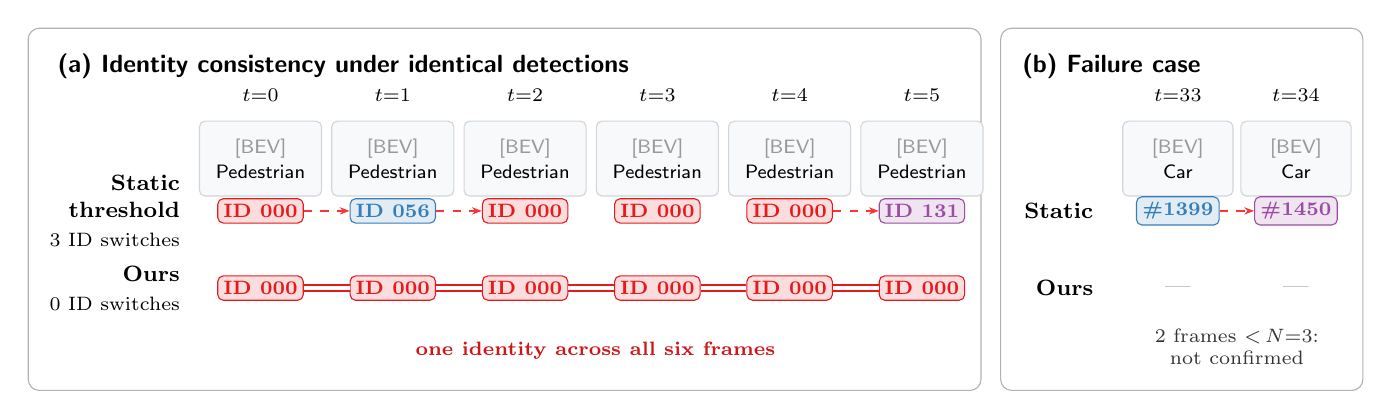
\begin{tikzpicture}[
    font=\small\sffamily,
    framebox/.style={draw=bordergray, fill=boxbg, rounded corners=2pt, minimum width=1.55cm, minimum height=0.95cm, align=center, inner sep=2pt},
    tagred/.style={fill=idred!15, text=idred, draw=idred, font=\scriptsize\bfseries, rounded corners=2pt, inner sep=2pt, minimum width=1.05cm, align=center},
    tagblue/.style={fill=idblue!15, text=idblue, draw=idblue, font=\scriptsize\bfseries, rounded corners=2pt, inner sep=2pt, minimum width=1.05cm, align=center},
    tagpurple/.style={fill=idpurple!15, text=idpurple, draw=idpurple, font=\scriptsize\bfseries, rounded corners=2pt, inner sep=2pt, minimum width=1.05cm, align=center},
    subpanel/.style={draw=black!30, fill=white, rounded corners=4pt}
]
% ---------------- panel (a) : 0 .. 12.2 ----------------
\node[anchor=north west, font=\small\sffamily] (titleA) at (0.25, -0.2) {\textbf{(a) Identity consistency under identical detections}};
\node[anchor=east, align=right, font=\footnotesize] (lblStaticA) at (2.05, -2.32) {\textbf{Static}\\\textbf{threshold}\\[1pt]{\scriptsize 3 ID switches}};
\node[anchor=east, align=right, font=\footnotesize] (lblOursA)   at (2.05, -3.30) {\textbf{Ours}\\[1pt]{\scriptsize 0 ID switches}};
\foreach \i/\t in {0/{$t{=}0$}, 1/{$t{=}1$}, 2/{$t{=}2$}, 3/{$t{=}3$}, 4/{$t{=}4$}, 5/{$t{=}5$}} {
    \node[anchor=center, font=\scriptsize\bfseries] (timeA\i) at (2.95 + \i*1.68, -0.85) {\t};
    \node[framebox, below=0.12cm of timeA\i] (frameA\i) {
        \textcolor{gray!80}{\scriptsize [BEV]}\\[-2pt]
        \scriptsize Pedestrian
    };
}
\node[tagred]    (s0) at (frameA0 |- lblStaticA) {ID 000};
\node[tagblue]   (s1) at (frameA1 |- lblStaticA) {ID 056};
\node[tagred]    (s2) at (frameA2 |- lblStaticA) {ID 000};
\node[tagred]    (s3) at (frameA3 |- lblStaticA) {ID 000};
\node[tagred]    (s4) at (frameA4 |- lblStaticA) {ID 000};
\node[tagpurple] (s5) at (frameA5 |- lblStaticA) {ID 131};
\draw[-{Stealth[length=3.5pt]}, dashed, red!80, line width=0.8pt] (s0) -- (s1);
\draw[-{Stealth[length=3.5pt]}, dashed, red!80, line width=0.8pt] (s1) -- (s2);
\draw[-{Stealth[length=3.5pt]}, dashed, red!80, line width=0.8pt] (s4) -- (s5);
\node[tagred] (o0) at (frameA0 |- lblOursA) {ID 000};
\node[tagred] (o1) at (frameA1 |- lblOursA) {ID 000};
\node[tagred] (o2) at (frameA2 |- lblOursA) {ID 000};
\node[tagred] (o3) at (frameA3 |- lblOursA) {ID 000};
\node[tagred] (o4) at (frameA4 |- lblOursA) {ID 000};
\node[tagred] (o5) at (frameA5 |- lblOursA) {ID 000};
\draw[double, double distance=1.2pt, idred, line width=0.9pt] (o0) -- (o1) -- (o2) -- (o3) -- (o4) -- (o5);
\node[anchor=center, font=\scriptsize\bfseries\color{idred!90!black}] (noteA) at (7.15, -4.10) {$\checkmark$ one identity across all six frames};
% ---------------- panel (b) : 12.45 .. 17.3 ----------------
\node[anchor=north west, font=\small\sffamily] (titleB) at (12.50, -0.2) {\textbf{(b) Failure case}};
\node[anchor=east, align=right, font=\footnotesize] (lblStaticB) at (13.65, -2.32) {\textbf{Static}};
\node[anchor=east, align=right, font=\footnotesize] (lblOursB)   at (13.65, -3.30) {\textbf{Ours}};
\node[anchor=center, font=\scriptsize\bfseries] (timeB0) at (14.60, -0.85) {$t{=}33$};
\node[anchor=center, font=\scriptsize\bfseries] (timeB1) at (16.10, -0.85) {$t{=}34$};
\node[framebox, minimum width=1.40cm, below=0.12cm of timeB0] (fb0) {\textcolor{gray!80}{\scriptsize [BEV]}\\[-2pt]\scriptsize Car};
\node[framebox, minimum width=1.40cm, below=0.12cm of timeB1] (fb1) {\textcolor{gray!80}{\scriptsize [BEV]}\\[-2pt]\scriptsize Car};
\node[tagblue,   minimum width=1.05cm] (sb0) at (fb0 |- lblStaticB) {\#1399};
\node[tagpurple, minimum width=1.05cm] (sb1) at (fb1 |- lblStaticB) {\#1450};
\draw[-{Stealth[length=3.5pt]}, dashed, red!80, line width=0.8pt] (sb0) -- (sb1);
\node[text=gray!70, font=\small] (ob0) at (fb0 |- lblOursB) {\textemdash};
\node[text=gray!70, font=\small] (ob1) at (fb1 |- lblOursB) {\textemdash};
\node[anchor=center, align=center, font=\scriptsize\color{black!80}] (noteB) at (15.35, -4.05) {2 frames ${<}\,N{=}3$:\\ not confirmed};
\begin{scope}[on background layer]
    \draw[subpanel] (0, 0) rectangle (12.10, -4.6);
    \draw[subpanel] (12.35, 0) rectangle (16.95, -4.6);
\end{scope}
\end{tikzpicture}
\caption{\textbf{Identity consistency under identical detections} (nuScenes \emph{val}, sensor frame, detection-budget-matched arms; dashed red arrows mark identity switches).
\textbf{(a)} One pedestrian in \texttt{scene-0925} over six consecutive keyframes. The emitted 3D box is identical in both arms in every frame --- same centre, size, orientation and score (0.726--0.833, centre error $\le 0.27$\,m, correctly classified throughout) --- so the two rows differ only in the identity attached to that box. The static score threshold assigns three distinct identities, returning to the first one in between; confirmation-based initialisation with retrospective emission assigns one.
\textbf{(b)} The corresponding cost: a correctly classified, well-localised car in \texttt{scene-0104} visible for only two keyframes, one short of the $N{=}3$ confirmation window. The threshold emits it, already split across two identities; our policy does not emit it at all.}
\label{fig:identity_consistency}
\end{figure*}

% Preamble requirements (main.tex already loads amsmath,amssymb,tikz,graphicx):
\usetikzlibrary{positioning, arrows.meta, backgrounds, fit}
%
% Drawn at 17.3cm == \textwidth (6.875in = 17.46cm), so NO \resizebox is used and
% every label typesets at its true point size. Do not wrap this in \resizebox.

\definecolor{idred}{HTML}{E41A1C}
\definecolor{idblue}{HTML}{377EB8}
\definecolor{idgreen}{HTML}{4DAF4A}
\definecolor{idpurple}{HTML}{984EA3}
\definecolor{boxbg}{HTML}{F8F9FA}
\definecolor{bordergray}{HTML}{D1D5DB}

\begin{figure*}[t]
\centering
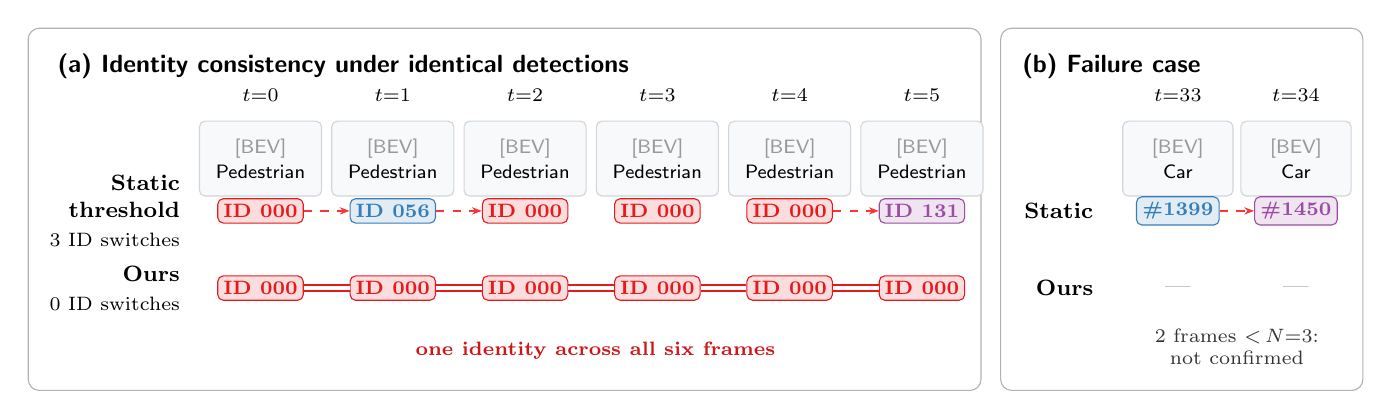
\begin{tikzpicture}[
    font=\small\sffamily,
    framebox/.style={draw=bordergray, fill=boxbg, rounded corners=2pt, minimum width=1.55cm, minimum height=0.95cm, align=center, inner sep=2pt},
    tagred/.style={fill=idred!15, text=idred, draw=idred, font=\scriptsize\bfseries, rounded corners=2pt, inner sep=2pt, minimum width=1.05cm, align=center},
    tagblue/.style={fill=idblue!15, text=idblue, draw=idblue, font=\scriptsize\bfseries, rounded corners=2pt, inner sep=2pt, minimum width=1.05cm, align=center},
    tagpurple/.style={fill=idpurple!15, text=idpurple, draw=idpurple, font=\scriptsize\bfseries, rounded corners=2pt, inner sep=2pt, minimum width=1.05cm, align=center},
    subpanel/.style={draw=black!30, fill=white, rounded corners=4pt}
]
% ---------------- panel (a) : 0 .. 12.2 ----------------
\node[anchor=north west, font=\small\sffamily] (titleA) at (0.25, -0.2) {\textbf{(a) Identity consistency under identical detections}};
\node[anchor=east, align=right, font=\footnotesize] (lblStaticA) at (2.05, -2.32) {\textbf{Static}\\\textbf{threshold}\\[1pt]{\scriptsize 3 ID switches}};
\node[anchor=east, align=right, font=\footnotesize] (lblOursA)   at (2.05, -3.30) {\textbf{Ours}\\[1pt]{\scriptsize 0 ID switches}};
\foreach \i/\t in {0/{$t{=}0$}, 1/{$t{=}1$}, 2/{$t{=}2$}, 3/{$t{=}3$}, 4/{$t{=}4$}, 5/{$t{=}5$}} {
    \node[anchor=center, font=\scriptsize\bfseries] (timeA\i) at (2.95 + \i*1.68, -0.85) {\t};
    \node[framebox, below=0.12cm of timeA\i] (frameA\i) {
        \textcolor{gray!80}{\scriptsize [BEV]}\\[-2pt]
        \scriptsize Pedestrian
    };
}
\node[tagred]    (s0) at (frameA0 |- lblStaticA) {ID 000};
\node[tagblue]   (s1) at (frameA1 |- lblStaticA) {ID 056};
\node[tagred]    (s2) at (frameA2 |- lblStaticA) {ID 000};
\node[tagred]    (s3) at (frameA3 |- lblStaticA) {ID 000};
\node[tagred]    (s4) at (frameA4 |- lblStaticA) {ID 000};
\node[tagpurple] (s5) at (frameA5 |- lblStaticA) {ID 131};
\draw[-{Stealth[length=3.5pt]}, dashed, red!80, line width=0.8pt] (s0) -- (s1);
\draw[-{Stealth[length=3.5pt]}, dashed, red!80, line width=0.8pt] (s1) -- (s2);
\draw[-{Stealth[length=3.5pt]}, dashed, red!80, line width=0.8pt] (s4) -- (s5);
\node[tagred] (o0) at (frameA0 |- lblOursA) {ID 000};
\node[tagred] (o1) at (frameA1 |- lblOursA) {ID 000};
\node[tagred] (o2) at (frameA2 |- lblOursA) {ID 000};
\node[tagred] (o3) at (frameA3 |- lblOursA) {ID 000};
\node[tagred] (o4) at (frameA4 |- lblOursA) {ID 000};
\node[tagred] (o5) at (frameA5 |- lblOursA) {ID 000};
\draw[double, double distance=1.2pt, idred, line width=0.9pt] (o0) -- (o1) -- (o2) -- (o3) -- (o4) -- (o5);
\node[anchor=center, font=\scriptsize\bfseries\color{idred!90!black}] (noteA) at (7.15, -4.10) {$\checkmark$ one identity across all six frames};
% ---------------- panel (b) : 12.45 .. 17.3 ----------------
\node[anchor=north west, font=\small\sffamily] (titleB) at (12.50, -0.2) {\textbf{(b) Failure case}};
\node[anchor=east, align=right, font=\footnotesize] (lblStaticB) at (13.65, -2.32) {\textbf{Static}};
\node[anchor=east, align=right, font=\footnotesize] (lblOursB)   at (13.65, -3.30) {\textbf{Ours}};
\node[anchor=center, font=\scriptsize\bfseries] (timeB0) at (14.60, -0.85) {$t{=}33$};
\node[anchor=center, font=\scriptsize\bfseries] (timeB1) at (16.10, -0.85) {$t{=}34$};
\node[framebox, minimum width=1.40cm, below=0.12cm of timeB0] (fb0) {\textcolor{gray!80}{\scriptsize [BEV]}\\[-2pt]\scriptsize Car};
\node[framebox, minimum width=1.40cm, below=0.12cm of timeB1] (fb1) {\textcolor{gray!80}{\scriptsize [BEV]}\\[-2pt]\scriptsize Car};
\node[tagblue,   minimum width=1.05cm] (sb0) at (fb0 |- lblStaticB) {\#1399};
\node[tagpurple, minimum width=1.05cm] (sb1) at (fb1 |- lblStaticB) {\#1450};
\draw[-{Stealth[length=3.5pt]}, dashed, red!80, line width=0.8pt] (sb0) -- (sb1);
\node[text=gray!70, font=\small] (ob0) at (fb0 |- lblOursB) {\textemdash};
\node[text=gray!70, font=\small] (ob1) at (fb1 |- lblOursB) {\textemdash};
\node[anchor=center, align=center, font=\scriptsize\color{black!80}] (noteB) at (15.35, -4.05) {2 frames ${<}\,N{=}3$:\\ not confirmed};
\begin{scope}[on background layer]
    \draw[subpanel] (0, 0) rectangle (12.10, -4.6);
    \draw[subpanel] (12.35, 0) rectangle (16.95, -4.6);
\end{scope}
\end{tikzpicture}
\caption{\textbf{Identity consistency under identical detections} (nuScenes \emph{val}, sensor frame, detection-budget-matched arms; dashed red arrows mark identity switches).
\textbf{(a)} One pedestrian in \texttt{scene-0925} over six consecutive keyframes. The emitted 3D box is identical in both arms in every frame --- same centre, size, orientation and score (0.726--0.833, centre error $\le 0.27$\,m, correctly classified throughout) --- so the two rows differ only in the identity attached to that box. The static score threshold assigns three distinct identities, returning to the first one in between; confirmation-based initialisation with retrospective emission assigns one.
\textbf{(b)} The corresponding cost: a correctly classified, well-localised car in \texttt{scene-0104} visible for only two keyframes, one short of the $N{=}3$ confirmation window. The threshold emits it, already split across two identities; our policy does not emit it at all.}
\label{fig:identity_consistency}
\end{figure*}
